\chapter{Background} % nothing of mine

% utrolig mye bra her: https://www.dei.unipd.it/\~emg/downloads/SIMPAR08-WorkshopProceedings/TeachingWithRobotics/karatrantou.pdf!! veldig mange bra kilder

% og mange eksempler herfra: https://student.cs.uwaterloo.ca/~cs231/resources/pseudocode.pdf

% mer på pseudokode: https://www.researchgate.net/profile/Nicholas-Bennett-6/publication/309410533\_Introduction\_to\_Algorithms\_and\_Pseudocode/links/60a489d04585158ca05c54bc/Introduction-to-Algorithms-and-Pseudocode.pdf

This chapter will cover concepts that one should be familiar with in order to fully understand the rest of this thesis. We start by providing a definition for pseudocode, to avoid confusion further down the line. We also discuss transpiling, how other transpilers work, and why Haskell is a good tool for the job.

\section{Pseudocode}

Pseudocode is a technique for describing computer programs in a more abstract way than programming languages allow, ignoring specific syntax and keywords. This can make programs easier to understand for both non-programmers and programmers alike, particularly when working with unfamiliar algorithms \cite{LinfoAlgorithmsIntro2007}. \hfill \\

Since it does not follow any precise syntax rules, pseudocode is subsequently not executable. This is not a bug, but rather a feature of pseudocode: it is intended for presenting ideas of code, not demonstrating results of code \cite{LogicsofSpecificationLanguages}. As such, pseudocode is an abstract concept, and can technically be anything, as long as it aims to aid others in understanding what a particular piece of code does. \hfill \\

When explaining a solution to a non-technical audience, the use of pseudocode is standard practice. Specifically, the pseudocode should encapsulate the crucial elements or the core functionality of the program. This focused presentation provides clarity on the essential aspects of the solution. Thus, even individuals without a programming background can provide feedback based on their understanding of the problem and its proposed solution. \hfill \\

Now, since pseudocode has many faces, we must define what we percieve pseudocode to be in the context of this thesis, and what exactly we mean when we refer to ``pseudocode'' in later parts of the thesis. To avoid further confusion, we will make a distinction between two particular types of pseudocode: text based- and image based pseudocode.

\subsection{Text based pseudocode}

The most common form of pseudocode is likely text based pseudocode (TBP), commonly found in text books on algorithms, published papers, as well as informal scribbling before attempting to solve a problem \cite{payAttentionToMLPs}\cite{BOOK:intro/Cormen/Leiserson}. It is also the form that most closely resembles source code, given that it usually includes line numbers, assign statements and generally presents the problem solution in an imperative matter \cite{proposalForParadigmGeneralPseudocode}. \hfill \\

Since there is no proper set of rules commanding how text based pseudocode should look like, we are prone to viewing different variations of the same algorithms across different literatures. A frequently presented algorithm is Binary Search, which in the context of computer science is a search algorithm that finds the position of a target value within a sorted array \cite{BOOK:intro/Cormen/Leiserson}. \hfill \\

In a note made for the Algorithmic Problem Solving course at the University of Waterloo, professor Naomi Nishimura has made a note\footnote{https://student.cs.uwaterloo.ca/~cs231/resources/pseudocode.pdf} where she presented four different variants of the Binary Search algorithm, all written in pseudocode. The algorithms are written with a total interval of 26 years from the oldest to the newest. \hfill \\

The oldest variant is from 1974, presented in The Design and Analysis of Computer Algorithms by Aho et al. \cite[139]{BOOK:DesignAnalysis/Aho}:

\begin{lstlisting}
    procedure SEARCH(a, f, l):
    if f $>$ l then return "no"
    else
        if a = A[$\lfloor$(f + l)/2$\rfloor$] then return "yes"
        else
            if a < A[$\lfloor$(f + l)/2$\rfloor$] then
                return SEARCH(a, f, $\lfloor$(f + l)/2$\rfloor$ - 1)
            else return SEARCH(a, $\lfloor$(f + l)/2$\rfloor$ + 1, l)
\end{lstlisting} \hfill \\

Then, roughly 17 years later, Lewis et al. present it like this in Data Structures and Their Algorithms \cite[182]{BOOK:DSA/Lewis}:

\begin{lstlisting}[basicstyle=\small\ttfamily]
    function BinarySearchLookUp(key K, table T[0..n-1]): info
    {Return information stored with key K in T, or $\Lambda$ if K is not in T}
        Left $\gets$ 0
        Right $\gets$ n - 1
        repeat forever
            if Right < Left then
                return $\Lambda$
            else
                Middle $\gets$ $\lfloor$(Left + Right) / 2$\rfloor$
                if K = Key(T[Middle]) then return Info(T[Middle])
                else if K < Key(T[Middle]) then Right $\gets$ Middle - 1
                else Left $\gets$ Middle + 1
\end{lstlisting}

The desire for automatic generation of TBP has been in the wind for some time, with the intention of presenting ideas without having to worry about syntax of a particular programming language \cite{desireToGetPseudocodeGeneration}. Text based pseudocode allows authors to draft ideas in an imperative way, just like we write recipes for baking bread and building legos. Here, the author is free to omit boilerplate code, include mathematical notation and necessary abstractions, and even resort to natural language where deemed appropriate \cite{BOOK:intro/Cormen/Leiserson}\cite{DBLP:conf/els/Nuallain15}. \hfill \\

As previously mentioned, pseudocode has a well-established history in university curricula. When learning algorithms, data structures, or programming concepts, the focus is really on the underlying ideas. These concepts are generally more important than the specifics of how they are implemented in a specific programming language. Thus, learning with TBP serves to maintain a similar level of abstraction, without demanding familiarity with a particular programming language. This approach prioritises concept comprehension over language-specific knowledge. \hfill \\

Freely available alternatives for transpiling source code to pseudocode is Code Kindle\footnote{https://devpost.com/software/code-kindle} and Pseudogen, a tool introduced by Oda et. al \cite{DBLP:conf/kbse/OdaFNHSTN15}. Both solutions use statistical machine translation, which is a technique to train a model on previously translated and analyzed information and conversations%\footnote{https://en.wikipedia.org/wiki/Statistical\_machine\_translation}
. With Pseudogen, code is transpiled to purely natural language. Code Kindle's results are less verbose, though in most cases still a description accompanying the original source code. \hfill \\

Its usefulness is also backed by the numerous other attempts at translating source code to TBP in the past \cite{PSEU:/Kreher/Stinson}\cite{DBLP:conf/aswec/AlhefdhiDHG18}.

\subsection{Image based pseudocode}

Not all programming languages share the same execution flow. For instance, in VHDL all processes are executed simultaneously\footnote{https://www.people.vcu.edu/~rhklenke/tutorials/vhdl/modules/m12\_23/sld008.htm}, whilst rewriting rules in Maude are applied non-deterministically (if multiple rules can apply to a term, any one of them may be chosen in an arbitrary order). Some languages, on the other hand, like Python, will execute their programs line for line. This means that we can follow the execution flow simply by looking at the order functions are called and the order of statements within those functions. \hfill \\

This way of executing a program opens up for the possibility of image based pseudocode (IBP), which still includes text, but also complements it with boxes, arrows and perhaps pretty colours. When code stretches over enough lines, code becomes uniform in appearance and challenging to differentiate. By contrast, IBP distinctively isolates each statement, providing more of a birds eye perspective on the program. \hfill \\

In fact, images in computer science is nothing new. One of the most notable examples we have are the ones we use for finite state automata (FSA). An FSA is a machine which either accepts or rejects a given string, by running each symbol through a state sequence uniquely determined by said string. We differentiate betwee deterministic and non-deterministic FSAs, though it is not of importance in our context. What they share, is a number of states, a start state, a transition function and an accept state \cite{introToAutomataTheory}. \hfill \\

\begin{figure}[ht]
    \centering
    \includegraphics[scale=0.46]{assets/dfa.png}
    \caption{An example finite state automata.}
    \label{fig:dfa}
\end{figure}

Figure 2.3 shows an example of an FSA which accepts the word ``pseudo'' followed by an arbitrary amount of exclamation marks. The FSA has 8 states, and the leftmost arrow indicates that \textbf{1} is the starting state. From here, we can get to the second state if our string starts with the symbol ``p''. Thus, all strings that do not begin with a ``p'' are rejected at this point. States 7 and 8 have an additional ring within their circle, which means that they are accepting states. If a combination of symbols have not been rejected at this point, and is finished, it is accepted. State 8 has an arrow leading to itself via the symbol ``!'', meaning that it can end with as many exclamation marks as possible. \hfill \\

A string like ``pseudo!!p!!!'' is not accepted, however, despite starting with ``pseudo!!'' and ending with ``!!!''. Once a string has reached state 8, it can \textit{only} be followed by exclamation marks, or else it is rejected. \hfill \\

Warren McCulloch and Walter Pitts were among the first researchers to introduce a concept similar to finite automata, all the way back in 1943 \cite{McCulloch43}. Their paper presents a simplified computational model of biological neurons. \hfill \\

Throughout the remainder of this thesis, when we talk about ``image based pseudocode'', we are referring to flowcharts. The title does not technically belong to flowcharts alone, but it is the way we will go about things. \hfill \\

There have also been multiple attempts at creating flowchart editors, most notably by Carlisle et al. and Charntaweekhun et al. \cite{carlisle2004}\cite{charntaweekhun2006}. These allows authors to visualise their ideas, rather than keeping it all text based. Benefits of learning with help from visual aid is well documented, which is one of the reasons introductory math books are always so colourful [kilde?]. \hfill \\ % It seems a stretch to believe that students could not benefit from learning with images also when it comes to algorithms and programming concepts. \hfill \\

One of few editors that generates flowcharts directly from code is Code2Flow\footnote{You can try the editor for free at https://app.code2flow.com/}. This is a DSL with support for most common programming concepts like statements, loops, conditionals, and more. The editor comes with a comprehensible guide on its syntax. It is also a highly customisable tool, letting you change the flowcharts' fonts, colours, sizes and even edge height. \hfill \\

\begin{figure}[ht]
    \centering
    \includegraphics[scale=0.46]{assets/fibonacci_flowchart.png}
    \caption{Image based pseudocode illustrating an algorithm to retrieve the nth number in a Fibonacci sequence, created with Code2Flow.}
    \label{fig:fibseq1}
\end{figure}

Given the imperative nature of flowcharts, the way they walk through problems step-by-step, there have also been attempts at converting image based pseudocode to text based pseudocode. Wu et al. proposed a structure identification algorithm, which can take an identified flowchart as input, and automatically generate code in return \cite{codeFromFlowcharts}. This gives even more ground to perceive flowcharts as an image based form of pseudocode. \hfill \\

There have been multiple studies documenting the preference for IBP when it comes to studying algorithms, already back in the 80s by Scanlan et al. He documented how his students overwhelmingly preferred structured flowcharts to pseudocode for comprehending algorithms. Using multiple algorithms of varying complexity, the students most notably indicated that the flowcharts took less time to comprehend, provided fewer errors in understanding, and reduced the number of times they had to look at the algorithms \cite{DBLP:journals/software/Scanlan89}. \hfill \\

In newer times, Nita et al. attempted to analyse student's understanding of algorithms with pseudocode and flowcharts. The students were subjected to algol-like TBP, and IBP. Their conclusion was that the students found it easier to understand the selected algorithms in image format, as compared to a text based approach \cite{Nita_2020}.

% Bra språk for å snakke om flowcharts: https://www.researchgate.net/publication/234805404_Flowchart_techniques_for_structured_programming

\subsection{LaTeX}

LaTeX is a document preparation system that is widely used for the production of scientific documents\footnote{In fact, this thesis is written in LaTeX, through the editor Overleaf.}. It is an open-source typesetting system recognized for its capabilities in creating visually appealing documents that meet typographic standards. \hfill \\

Unlike traditional word processors like Microsoft Word or Google Docs, LaTeX operates more similarly to how we write code. The user typesets the document in plain text, with various commands that describe its structure and presentation. All documents must have a ``document class'', which is a set of formatting instructions that dictate how a document will look. Additionally, all content in a LaTeX file must be within the commands ``\textbackslash begin\{document\}'' and ``\textbackslash end\{document\}''. \hfill \\

LaTeX builds upon the TeX typesetting system created by Donald Knuth. It added a collection of macros that simplified the use of TeX, and made it more accessible to non-technical users. \hfill \\

A distributed collection of macros in LaTeX is called a \textbf{package}. They allow users to add functionality or modify the behaviour of LaTeX, including refining typography, changing the layout of elements, creating graphics and more. In LaTeX documents, they are included using the \textbf{\textbackslash usepackage\{\}} command, and placed before \textbf{\textbackslash begin\{document\}}. \hfill \\

For this thesis, there are two LaTeX packages that are central: \textbf{Algorithm2e} and \textbf{TikZ}. Algorithm2e is a package to typeset algorithms or pseudocode. TikZ, on the other hand, is probably the most complex and powerful tool to create graphic elements in LaTeX. In this thesis, Algorithm2e will be used for TBP and TikZ for IBP. \hfill \\

Algorithm2e provides an algorithm environment you can access through \\ \textbf{\textbackslash begin\{algorithm2e\}}\footnote{https://www.overleaf.com/learn/latex/Algorithms\#The\_algorithm2e\_package}. TikZ provides an environment you can access through \textbf{\textbackslash begin\{tikzpicture\}}\footnote{https://www.overleaf.com/learn/latex/TikZ\_package}. We must also remember to include \\ \textbf{\textbackslash usepackage\{algorithm2e\}} and \textbf{\textbackslash usepackage\{tikz\}} in our preamble. \hfill \\

A simple TBP example with Algorithm2e is provided in footonte 6. An identifier ``i'' is declared, and a nested control sequence is defined.

\begin{algorithm}
$i\gets 10$\;
\eIf{$i\geq 5$}
{
    $i\gets i-1$\;
}{
    \If{$i\leq 3$}
    {
        $i\gets i+2$\;
    }
}
\end{algorithm}

In footnote 7 we are introduced to a small example of IBP with TikZ. We see a flow going from one circle, passing two rectangles and ending on another circle. The path is denoted by arrows.

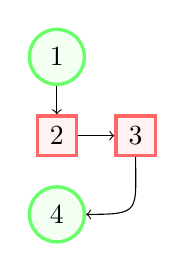
\begin{tikzpicture}[
roundnode/.style={circle, draw=green!60, fill=green!5, very thick, minimum size=7mm},
squarednode/.style={rectangle, draw=red!60, fill=red!5, very thick, minimum size=5mm},
]
%Nodes
\node[squarednode] (maintopic) {2};
\node[roundnode] (uppercircle) [above of=maintopic] {1};
\node[squarednode] (rightsquare) [right of=maintopic] {3};
\node[roundnode] (lowercircle) [below of=maintopic] {4};

%Lines
\draw[->] (uppercircle.south) -- (maintopic.north);
\draw[->] (maintopic.east) -- (rightsquare.west);
\draw[->] (rightsquare.south) .. controls +(down:7mm) and +(right:7mm) .. (lowercircle.east);
\end{tikzpicture}

\section{Transpiling}

The reader might be familiar with the concept of \textit{compiling}. Traditionally, this is a process where a \textit{compiler} reads a program in a high-level language and translates it to an executable target program \cite{DBLP:books/aw/AhoSU86}. \hfill \\

A transpiler, however, is a tool that converts input source code into output source code, maintaining a similar abstraction level \cite{DBLP:conf/els/MarcelinoL22}. The first transpiler to our knowledge was developed in 1978 by Intel, with the aim of translating assembly source code from the 8080/8085 processor to the 8086 processor \cite{intel1979}. \hfill \\

An example of transpiling involves the JavaScript programming language\footnote{https://developer.mozilla.org/en-US/docs/Web/JavaScript/Language\_overview}, commonly used in web development. It is a language in constant development, frequently updating its features. The issue with this is that not all browsers are always compatible with its newest features. Therefore, there exists a transpiler Babel\footnote{https://babeljs.io} which converts modern JavaScript into a backwards compatible version. According to Nicolini et al., without a transpiler almost 14\% of web users risk facing a JavaScript bug when accessing a website with new JavaScript features \cite{DBLP:journals/software/NicoliniHF24}. \hfill \\

Another example is a transpiler presented by Lunnikiv etl. al, where Python is converted to Rust as an intermediate source code step. The paper shows how pre-existing Python implementations that depend on optimised libraries can be transpiled to Rust semi-automatically \cite{DBLP:conf/samos/LunnikiviJ020}. This way, the user can keep writing Python, whilst additionally allowing for the performance optimisation given by Rust.

\subsection{Generators}

Given how syntactically rich programming languages tend to be (in that they tend to have many keywords etc), it seems like too difficult of a task to have 1-to-1 mappings from the input source language to the output source language. There are infinite combinations of programs we can write[kilde?], thus we could benefit from some sort of intermediate representation. One of these methods is using so-called \textit{generators}. \hfill \\

A generator is basically a stand-alone parser or writer. A parser generator translates a program written in a source language to an abstract syntax tree (AST). A writer generator translates an AST to a program in a target language. \hfill \\

There are several benefits of using generators. One of them is flexibility. Generators can handle a wide range of source code structures and translate them into various target languages. Another one is naturally the modularity. If we wish to add another reader, we can simply implement one and put it ``on top'' of the rest, without having to modify anything else. Thus we only need to maintain our reader if we wish to change the representation. \hfill \\

An example of this is the programming language Derw\footnote{https://github.com/eeue56/derw}, an ML language mainly inspired by Elm. By utilising generators\footnote{https://github.com/eeue56/derw/tree/main/src/generators}, it has multiple writers, among others bytecode, JavaScript, and even English. Figure 2.5 shows how expressions like $6 <= 8$ are translated. The token \textbf{lessThanOrEqual} has a left- and right pointer, corresponding to the respective integers. These are extracted, and put on each side of the string ``is less than or equal to''. \hfill \\

% Change this to light mode?
\begin{figure}[ht]
    \centering
    \includegraphics[scale=0.7]{assets/derwLTE.png}
    \caption[]{An excerpt from the english generator in Derw, showing how expressions with ``less than or equal'' are converted\footnotemark.}
    \label{fig:derw}
\end{figure}
\footnotetext{https://github.com/eeue56/derw/blob/main/src/generators/English.derw}

Another example is Pandoc, which works with markdown languages. It has a ``core language'' which all parsers and writers must work with:

\begin{verbatim}
    Plain [Inline]
    Para [Inline]
    LineBlock [[Inline]]
    CodeBlock Attr String
    RawBlock Format String
    BlockQuote [Block]
    OrderedList ListAttributes [[Block]]
    BulletList [[Block]]
    DefinitionList [([Inline], [[Block]])]
    Header Int Attr [Inline]
    HorizontalRule
    Table [Inline] [Alignment] [Double] [TableCell] [[TableCell]]
    Div Attr [Block]
    Null
\end{verbatim}

% [kilde]

Every inputlanguage must be able to parse to (at least) these data types, and every writer must be able to work with these data types. However, writing a document in a rich format like Latex, and later converting it to a different markup language might tends to pose problems due to the different philosophies that underlie each language. Yet Pandoc is an excellent interpreter of lightweight markup languages like Markdown, which are ``neutural'' by design \cite{dominici2014}.

\subsection{Haskell's strengths}
As previously mentioned, we opted for the Haskell programming language when implementing Psnodig. There are several reasons as to why, but the primary one is that it is widely perceived as a fitting tool when working with programming languages, and particularly when working with interpreters\footnote{https://github.com/Gabriella439/post-rfc/blob/main/sotu.md\#compilers}. At the end of the day, programming languages are just tools, and we believe this is the best one for this particular job. \hfill \\

With Haskell, it is straightforward to create your own \textbf{data types}, which are then used to model ASTs. For instance, we can create our own calculator language in just a few lines of code:

\begin{verbatim}
    data Program = Program Expression

    data Expression =
          CompoundExpression Integer Operator Expression
        | IntExpression Integer

    data Operator =
          Plus
        | Minus
        | Times
        | Division
\end{verbatim}

From this, we can construct the following AST:

\begin{verbatim}
    Program (CompoundExpression 1 Plus
                (CompoundExpression 2 Minus
                    (IntExpression 3))
\end{verbatim}

As you can also see, we could create much bigger calculations than this. If we wish to expand our operators data type (with for instance an exponent), we only have to add a pipe and the operator name, like so:

\begin{verbatim}
    data Operator =
          Plus
        | Minus
        | Times
        | Division
        | Exponent
\end{verbatim}

Another benefit of using Haskell, is that its strong type system opens for clean and efficient pattern matching. This is very useful, both when writing the interpreter, but also when adding new, potential readers. For instance, if we wish to transpile the above AST to text, we could start with writing a function to convert the operators:

\begin{lstlisting}[caption={Haskell example to convert data type to string}, captionpos=b]
    f :: Operator -> String
    f (Operator Plus)     = " + "
    f (Operator Minus)    = " - "
    f (Operator Times)    = " / "
    f (Operator Division) = " * "
\end{lstlisting}

The function \textbf{f} takes something of type \textbf{Operator} as input, and returns something of type \textbf{String}. It will pattern match on the input, and return a correspondng value, making it bijective. We could add case of \texttt{f \_ = ""}, which would return the empty string for any other kind of operator, though this would be redundant as we have not defined any other type of operator anyway. \hfill \\

Lastly, we can utilise the QuickCheck\footnote{https://hackage.haskell.org/package/QuickCheck}, which is a testing library suited for automatic property-based testing in Haskell. With this we can prove different properties of our tool \cite{DBLP:conf/icfp/ClaessenH00}, and perhaps also of other (primarily) parsers and (maybe) writers, given that they have to pass through Haskell ADTs anyway.